\documentclass[]{article}
\usepackage{lmodern}
\usepackage{amssymb,amsmath}
\usepackage{ifxetex,ifluatex}
\usepackage{fixltx2e} % provides \textsubscript
\ifnum 0\ifxetex 1\fi\ifluatex 1\fi=0 % if pdftex
  \usepackage[T1]{fontenc}
  \usepackage[utf8]{inputenc}
\else % if luatex or xelatex
  \ifxetex
    \usepackage{mathspec}
  \else
    \usepackage{fontspec}
  \fi
  \defaultfontfeatures{Ligatures=TeX,Scale=MatchLowercase}
\fi
% use upquote if available, for straight quotes in verbatim environments
\IfFileExists{upquote.sty}{\usepackage{upquote}}{}
% use microtype if available
\IfFileExists{microtype.sty}{%
\usepackage{microtype}
\UseMicrotypeSet[protrusion]{basicmath} % disable protrusion for tt fonts
}{}
\usepackage[margin=1in]{geometry}
\usepackage{hyperref}
\hypersetup{unicode=true,
            pdftitle={Regime Switching and Technical Trading with Dynamic Bayesian Networks in High-Frequency Stock Markets},
            pdfauthor={Luis Damiano, Brian Peterson, Michael Weylandt},
            pdfborder={0 0 0},
            breaklinks=true}
\urlstyle{same}  % don't use monospace font for urls
\usepackage{natbib}
\bibliographystyle{plainnat}
\usepackage{longtable,booktabs}
\usepackage{graphicx,grffile}
\makeatletter
\def\maxwidth{\ifdim\Gin@nat@width>\linewidth\linewidth\else\Gin@nat@width\fi}
\def\maxheight{\ifdim\Gin@nat@height>\textheight\textheight\else\Gin@nat@height\fi}
\makeatother
% Scale images if necessary, so that they will not overflow the page
% margins by default, and it is still possible to overwrite the defaults
% using explicit options in \includegraphics[width, height, ...]{}
\setkeys{Gin}{width=\maxwidth,height=\maxheight,keepaspectratio}
\IfFileExists{parskip.sty}{%
\usepackage{parskip}
}{% else
\setlength{\parindent}{0pt}
\setlength{\parskip}{6pt plus 2pt minus 1pt}
}
\setlength{\emergencystretch}{3em}  % prevent overfull lines
\providecommand{\tightlist}{%
  \setlength{\itemsep}{0pt}\setlength{\parskip}{0pt}}
\setcounter{secnumdepth}{5}
% Redefines (sub)paragraphs to behave more like sections
\ifx\paragraph\undefined\else
\let\oldparagraph\paragraph
\renewcommand{\paragraph}[1]{\oldparagraph{#1}\mbox{}}
\fi
\ifx\subparagraph\undefined\else
\let\oldsubparagraph\subparagraph
\renewcommand{\subparagraph}[1]{\oldsubparagraph{#1}\mbox{}}
\fi

%%% Use protect on footnotes to avoid problems with footnotes in titles
\let\rmarkdownfootnote\footnote%
\def\footnote{\protect\rmarkdownfootnote}

%%% Change title format to be more compact
\usepackage{titling}

% Create subtitle command for use in maketitle
\newcommand{\subtitle}[1]{
  \posttitle{
    \begin{center}\large#1\end{center}
    }
}

\setlength{\droptitle}{-2em}
  \title{Regime Switching and Technical Trading with Dynamic Bayesian Networks in
High-Frequency Stock Markets}
  \pretitle{\vspace{\droptitle}\centering\huge}
  \posttitle{\par}
  \author{Luis Damiano, Brian Peterson, Michael Weylandt}
  \preauthor{\centering\large\emph}
  \postauthor{\par}
  \predate{\centering\large\emph}
  \postdate{\par}
  \date{2017-08-26}

\usepackage[linesnumbered,ruled,vlined]{algorithm2e}
\usepackage{bm} % True bold symbols
\usepackage{float} % Image position
\usepackage{tabularx} % Tables
\usepackage{tikz} % Graphs
\usetikzlibrary{positioning}

% Math operators
\DeclareMathOperator*{\argmax}{\operatorname*{arg\,max}}
\DeclareMathOperator*{\argmin}{\operatorname*{arg\,min}}
\DeclareMathOperator{\evsym}{E}
\newcommand\ev[1]{\evsym\left\langle#1\right\rangle}
\DeclareMathOperator{\vsym}{V}
\newcommand\vv[1]{\vsym\left\langle#1\right\rangle}

% Math commands
\newcommand{\mat}[1]{\bm{#1}}

% Math symbols
\newcommand{\NN}{\mathbb{N}}
\newcommand{\LL}{\mathcal{L}}
\newcommand{\RR}{\mathbb{R}}

\usepackage{lscape}
\newcommand{\blandscape}{\begin{landscape}}
\newcommand{\elandscape}{\end{landscape}}

\begin{document}
\maketitle

{
\setcounter{tocdepth}{2}
\tableofcontents
}
This work aims at \ldots{} .

The authors acknowledge Google for financial support via the Google
Summer of Code 2017 program.

\begin{center}\rule{0.5\linewidth}{\linethickness}\end{center}

\section{Motivation}\label{motivation}

\section{Hierarchical Hidden Markov
Models}\label{hierarchical-hidden-markov-models}

The Hierarchical Hidden Markov Model (HHMM) is a recursive hierarchical
generalization of the HMM that provides a systematic unsupervised
approach for complex multi-scale structure. The model is motivated by
the multiplicity of length scales and the different stochastic levels
(recursive nature) present in some sequences. Additionally, it infers
correlated observations over long periods via higher levels of
hierarchy.

The model structure is fairly general and allows an arbitrary number of
activations of its submodels. The multi-resolution structure is handled
by temporal experts\footnote{In Machine Learning terminology, a problem
  is divided into homogeneous regions addressed by an expert submodel. A
  gating network or function decides which expert to use for each input
  region.} of different time scales.

\subsection{Model specification}\label{model-specification}

HHMM are structured multi-level stochastic processes that generalize HHM
by making each of the hidden states an autonomous probabilistic model.
There are two kinds of states: internal states are HHMM that emit
sequences by a recursive activation of one of the substates, while
production states generate an output symbol according to the probability
distribution of the set of output symbols.

Hidden dynamics are lead by transitions. Vertical transitions involve
the activation of a substate by an internal state, they may include
further vertical transitions to lower level states. Once completed, they
return the control to the state that originated the recursive activation
chain. Then, a horizontal transition is performed. Its state transition
within the same level.

A HHMM can be represented as a standard single level HMM whose states
are the production states of the corresponding HHMM with a fully
connected structure, i.e.~there is a non-zero probability of tranisition
from any state to any other state. This equivalent new model lacks the
multi-level structure.

Let \(z_{t}^{d} = i\) be the state of an HHMM at the step \(t\), where
\(i \in \{1, \dots, |z^{d}|\}\) is the state index, \(|z^{d}|\) is the
number of possible steps within the \(d\)-th level and
\(d \in \{1, \dots, D\}\) is the hierarchy index taking values \(d = 1\)
for the root state, \(d = \{2, \dots, ..., D-1\}\) for the remaining
internal states and \(d = D\) for the production states.

In addition to its structure, the model is characterized by the state
transition probability between the internal states and the output
distribution of the production states. For each internal state \(z_t^d\)
for \(d \in \{1, \dots, D - 1\}\), there is a state transition
probability matrix \(\mat{A}^d\) with elements
\(A_{ij}^{d} = p(z_{t}^{d+1} = j | z_{t}^{d+1} = j)\) is the probability
of a horizontal transition from the \(i\)-th state to the \(j\)-th state
within the level \(d\). Similarly, there is the initial distribution
vector over the substates \(\mat{\pi}^d\) with elements
\(\pi_j^d = p(z_t^{d+1} = j | z_t^d)\) for
\(d \in \{1, \dots, D - 1\}\). Finally, each production state \(z_t^D\)
is parametrized by the output parameter vector \(\mat{\theta}_o^i\)
whose form depends on the specification of the observation model
\(p(\mat{x}_t | z_t^D = j, \mat{\theta}_o^j)\) corresponding to the
\(j\)-th production state.

\subsection{Generative model}\label{generative-model}

The root node initiates a stochastic sequence generation. An observation
for the first step in the sequence \(t\) is generated by drawing at
random one of the possible substates according to the initial state
distribution \(\mat{\pi}^1\). To replicate the recursive activation
process, for each internal state entered \(z_t^d\) one of the substates
is randomly chosen according to the corresponding initial probability
vector \(\mat{\pi}^d\). When an internal state transitions to a
production state \(z_t^D = j\), a single observation is generated
according to the state output parameter vector \(\mat{\theta}_o^j\).
Control returns to the internal state that lead to the current
production state \(z_t^{D-1}\), which in turns selects the next state in
the same level according to transition matrix \(\mat{A}^{D-1}\).

Save for the top, each level \(d \in \{2, \dots, D\}\) has a final state
that terminates the stochastic state activation process and returns the
control to the parent state of the whole hierarchy. The generation of
the observation sequence is completed when control of all the recursive
activations returns to the root state.

\subsection{Parameter estimation}\label{parameter-estimation}

The parameters of the models are
\(\mat{\theta} = \left\{ \left\{ \mat{A}^d \right\}_{d \in \{1, \dots, D - 1\}}, \left\{ \mat{\pi}^d \right\}_{d \in \{1, \dots, D - 1\}}, \left\{ \mat{\theta}_o \right\} \right\}\).
The form of \(\mat{\theta}_o\) depends on the specification of the
production states. We refer the read to \citet{fine1998hierarchical} for
a detailed treatment of estimation and inference procedures.

\begin{center}\rule{0.5\linewidth}{\linethickness}\end{center}

\section{Regime Switching and Technical Trading with Dynamic Bayesian
Networks in High-Frequency Stock
Markets}\label{regime-switching-and-technical-trading-with-dynamic-bayesian-networks-in-high-frequency-stock-markets}

\subsection{Preamble}\label{preamble}

\ldots{}

\subsection{Feature extraction}\label{feature-extraction}

\subsubsection{Input series}\label{input-series}

Tick series are a sequence of triples \(\{y_k\}\) with
\(y_k = (t_k, p_k, v_k)\), where \(t_k \le t_{k+1}\) is the time stamp
in seconds, \(p_k\) is the trade price and \(v_k\) is the trade volume.
The sequence is ordered by the occurence of trades. There can be more
than one trade within a second.

Following \citet{tayal2009regime}, who in turns drew inspiration from
the technical analysis techniques proposed by \citet{ord2008secret}, we
derive a zig-zag sequence that captures the bid-ask bounce \(\{z_k\}\)
with \(z_k = (i_n, j_n, e_n, \phi_n)\), where \(i_n \le i_j\) are
indices to the tick series representing the starting and ending point of
the extrema, \(e_n = p_k \ \forall \ k : i_n \le k \le j_n\) is the
price at the local extrema, and \(\phi_m\) measures the average volume
per second during the zig-zag leg ending at \(e_n\):

\[
\phi_n = \frac{1}{t_{j_n} - t_{i_{n-1}} + 1} \sum_{k = i_{n-1}}^{j_n}{v_k}.
\]

We note that \(p_{i_n} < e_n < p_{j_n + 1}\) for local maxima and
\(p_{i_n} > e_n > p_{j_n + 1}\) for local minima. The average volume,
which includes the end-point extrema, is normalized by
\(t_{j_{n}} - t_{i_{n-1}} + 1\) to avoid division by zero when the
zig-zag leg occurs within the same time period. Most importantly, we
underline that the \(n\)-th zig-zag point \(z_n\) is realized only after
observing the \((j_n + 1)\)-th tick point \(y_{j_n + 1}\). Failing to
consider the one tick lag between leg completion and the time of
detection would cause look-ahead bias in the out of sample forecasts.

\subsubsection{Processing rules}\label{processing-rules}

Discrete features are created based on the zig-zag series \(\{z_n\}\).
We first create an auxiliary series \(\{O_n\}\) with
\(O_n = (f_n^0, f_n^1, f_n^2)\), where \(f_n^0\) represents the
direction of the zig-zag, \(f_n^1\) indicates the existence of a trend
and \(f_n^2\) indicates whether average volume increased or decreased.

Formally,

\[
f_n^0 =
\begin{cases}
+1 & \text{if $e_n$ is a local maximum (positive zig-zag leg)} \\
-1 & \text{if $e_n$ is a local minimum (negative zig-zag leg),} \\
\end{cases}
\]

and

\[
f_n^1 =
\begin{cases}
+1 & \text{if $e_{n-4} < e_{n-2} < e_{n} \wedge e_{n-3} < e_{n-1}$ (up-trend)} \\
-1 & \text{if $e_{n-4} > e_{n-2} > e_{n} \wedge e_{n-3} > e_{n-1}$ (down-trend)} \\
 0 & \text{otherwise (no trend).}
\end{cases}
\]

For the third indicator function, we compute the average volume ratios,

\[
\nu_n^1 = \frac{\phi_n}{\phi_{n-1}}, \quad \nu_n^2 = \frac{\phi_n}{\phi_{n-2}}, \quad \nu_n^1 = \frac{\phi_{n-1}}{\phi_{n-2}},
\]

we transform the ratios into a discrete variable using an arbitrary
threshold \(\alpha\),

\[
\tilde{\nu}_n^j =
\begin{cases}
+1 & \text{if $\nu_n^j - 1 > \alpha$} \\
-1 & \text{if $1 - \nu_n^j > \alpha$} \\
 0 & \text{if $|\nu_n^j - 1| \le \alpha$}, \\
\end{cases}
\]

and we finallly define

\[
f_n^2 =
\begin{cases}
+1 & \text{if $\tilde{\nu}_n^1 = 1, \tilde{\nu}_n^2 > -1, \tilde{\nu}_n^3 < 1$ (volume strengthens)} \\
-1 & \text{if $\tilde{\nu}_n^1 = -1, \tilde{\nu}_n^2 < -1, \tilde{\nu}_n^3 > -1$ (volume weakens)} \\
 0 & \text{otherwise (volume is indeterminant)}. \\
\end{cases}
\]

The features or legs \(\mat{D} = \{D_1, \dots, D_9 \}\),
\(\mat{U} = \{U_1, \dots, U_9 \}\) are then created using the table
\(\ref{tab:feature-space}\).

\% latex table generated in R 3.3.3 by xtable 1.8-2 package \% Sat Aug
26 14:09:52 2017

\begin{table}[ht]
\centering
\begingroup\footnotesize
\begin{tabularx}{0.7 \textwidth}{rrrrr}
  \toprule
 & Zig-zag direction & Price trend & Change in volume & Market State \\ 
  \midrule
$D_{1}$ & Down -1 & Up +1 & dn & Bull \\ 
  $D_{2}$ & Down -1 & Down -1 & dn & Bull \\ 
  $D_{3}$ & Down -1 & Up +1 & Intederminant 0 & Bull \\ 
  $D_{4}$ & Down -1 & No trend & dn & Bull \\ 
  $D_{5}$ & Down -1 & No trend & Intederminant 0 & Local volatility \\ 
  $D_{6}$ & Down -1 & No trend & Strong +1 & Bear \\ 
  $D_{7}$ & Down -1 & Down -1 & Intederminant 0 & Bear \\ 
  $D_{8}$ & Down -1 & Up +1 & Strong +1 & Bear \\ 
  $D_{9}$ & Down -1 & Down -1 & Strong +1 & Bear \\ 
   \midrule
$U_{1}$ & Up +1 & Up +1 & Strong +1 & Bull \\ 
  $U_{2}$ & Up +1 & Down -1 & Strong +1 & Bull \\ 
  $U_{3}$ & Up +1 & Up +1 & Intederminant 0 & Bull \\ 
  $U_{4}$ & Up +1 & No trend & Strong +1 & Bull \\ 
  $U_{5}$ & Up +1 & No trend & Intederminant 0 & Local volatility \\ 
  $U_{6}$ & Up +1 & No trend & dn & Bear \\ 
  $U_{7}$ & Up +1 & Down -1 & Intederminant 0 & Bear \\ 
  $U_{8}$ & Up +1 & Up +1 & dn & Bear \\ 
  $U_{9}$ & Up +1 & Down -1 & dn & Bear \\ 
   \bottomrule
\multicolumn{4}{l}{}\\
\end{tabularx}
\endgroup
\end{table}

Defining appropiate rules that capture trade volume dynamics and
identify trends in volume despite high-frequency noise is the most
challenging aspect of this design. \citet{wisebourt2011hierarchical}
proposes a modification for the feature extraction procedure. By
computing the spread between the Volume Weighted Average Prices of the
bid and the ask, he designs a book imbalance metric that describes the
state of the order book at any given moment in time. In turns,
\citet{sandoval2015computational} applies wavelets over two
simple-smoothed exponential distance-weighted average volume series to
measure trade volume concentration in both sides of the book.

\subsection{Model}\label{model}

\label{sec:model}

We adhere to the methodology proposed in the original work as much as
possible. We set up a HHMM to learn the sequence of discrete features
extracted from a high-frequency time series of stock prices and traded
volume. The figure below summarises the model structure in the form of a
Dynamic Bayesian Network.

The graph starts with a root node \(z^0\) that has two top-level
children \(z_1^1\) and \(z_2^1\) representing bullish markets (or runs)
and bearish markets (or reversals). The specifications do not pose any
constraints to determine beforehand which node takes each of the
possible two meanings. In consequence, latent states need to be labeled
after the learning stage based on sample characteristics such as mean
returns. Althought the original author does not mention this
possibility, prior information, like parameter ordering, could be
embedded to break symmetry and mitigate eventual identification issues.

\definecolor{myred}{RGB}{228, 31, 38}

\begin{figure}[!h]
\centering
\begin{tikzpicture}[
roundnode/.style={circle, draw=myred, very thick, minimum size=7mm},
groundnode/.style={circle, draw=myred, fill=myred!10, very thick, minimum size=7mm},
droundnode/.style={circle, double, draw=myred, very thick, minimum size=7mm},
]
%Nodes
\node[roundnode]                    (root)  {$z^0$};
\node[roundnode]                    (top1)  [below left  = 1.0cm and 1.5cm of root] {$z^1_1$};
\node[roundnode]                    (top2)  [below right = 1.0cm and 1.5cm of root] {$z^1_2$};
\node[groundnode, label={\small -}] (bot1)  [below left  = 1cm of top1] {$z^2_1$};
\node[groundnode, label={\small +}] (bot2)  [right       = 0.4cm of bot1] {$z^2_2$};
\node[droundnode]                   (bot51) [below right = 1cm of top1] {$z^2_5$};
\node[groundnode, label={\small +}] (bot3)  [below left  = 1cm of top2] {$z^2_3$};
\node[groundnode, label={\small -}] (bot4)  [right       = 0.4cm of bot3] {$z^2_4$};
\node[droundnode]                   (bot52) [below right = 1cm of top2] {$z^2_5$};

%Lines
\draw[->, dashed] (root) -- (top1);
\draw[->, dashed] (root) -- (top2);
\draw[->]         (top1) edge [bend right = 05] (top2);
\draw[->]         (top2) edge [bend right = 05] (top1);
\draw[->, dashed] (top1) -- (bot1);
\draw[->, dashed] (bot51) -- (top1);
\draw[->]         (bot1) edge [bend right = 10] (bot2);
\draw[->]         (bot2) edge [bend right = 10] (bot1);
\draw[->, dashed] (top2) -- (bot3);
\draw[->, dashed] (bot52) -- (top2);
\draw[->]         (bot3) edge [bend right = 10] (bot4);
\draw[->]         (bot4) edge [bend right = 10] (bot3);

\draw[->]         (bot1) edge [bend right = 60] (bot51);
\draw[->]         (bot3) edge [bend right = 60] (bot52);
\end{tikzpicture}
\caption{Hierarchical Hidden Markov Model for price and volumen proposed by @tayal2009regime.}
\end{figure}

Each top node activates a probabilistic HMM with two latent states for
negative and positive zig-zag legs. The sub-model activated by the node
\(z_1^1\) always starts with the node \(z_1^2\) producing an observation
from the distribution of negative zig-zag
\(\mat{D} = \{D_1, \dots, D_9 \}\). Next, it transitions to (a) the node
\(z_2^2\) producing a positive zig-zag leg
\(\mat{U} = \{U_1, \dots, U_9 \}\), (b) the end node which may, in turn,
transition back to \(z_1^1\) emitting a new negative zig-zag leg, or (c)
the end node and switches to the second sub-model, landing on node
\(z_3^2\) and producing a positive zig-zag leg. Restricting transitions
to this limited set of movements force alternation between positive and
negative zig-zag legs, thus guaranteeing that all possible observation
sequences are well behaved. The sub-model belonging to \(z_2^1\) has
similar but symmetrical behaviour. These two inner models are
conditionally independent, an advantage we will take for computational
time.

The persistence of price trends vary according to the resolution of the
dataset. In low frequency contexts, financial analysts will frequently
define short and long term trends based on timespans involving weeks and
months of observations. In high frequency trading, however, trends may
last from seconds to hours. The main idea behind the conception of the
hierarchical model is that top levels may group a sequence of price
movements forming a general trend, whereas the bottom nodes allow
zig-zags to represent micro trends that may deviate shortly from the
main drift. That is, the model accommodates for possibly unequally
probable negative price movements in an upwards market as well as
positive short trends in a price reversal.

Theoretically, all HHMM can be expressed as an equivalent HMM with
possibly sparse initial probability vector and transition matrix.
Although learning from this representation may prove less efficient in
terms of computational complexity, the relatively simple structure and
many restrictions of the model under study make estimation and inference
feasible. The equivalent ``expanded'' HMM has \(K = 4\) states, the
following \(K\)-sized initial probability vector

\[
\mat{\pi} = 
  \begin{bmatrix}
  \pi_1 & 0 & 1 - \pi_1 & 0 \\
  \end{bmatrix}
\]

and the \(K \times K\) transition matrix

\[
\mat{A} =
  \begin{bmatrix}
    0      & a_{12} & 1 - a_{11} & 0          \\
    1      & 0      & 0          & 0          \\
    a_{31} & 0      & 0          & 1 - a_{31} \\
    0      & 0      & 1          & 0          \\
  \end{bmatrix},
\]

where each element \(a_{ij}\) represents the probability of
transitioning from the hidden state \(i\) (row) to \(j\) (column) in one
step. The matrix is sparse with zeros representing nodes with no direct
connections. Since the initial probability vector and the rows of the
transition matrix must sum to \(1\), hidden dynamics are governed by
only three free parameters.

Production nodes emit one observation from the finite sets of possible
outputs \(\mat{O}_D\) (for \(z_1^2\) and \(z_4^2\)) and \(\mat{O}_U\)
(for \(z_2^2\) and \(z_3^2\)). Conditional probability distributions are
given by output probability vectors of length \(L = 9\) subject to
sum-to-one constraints:

\[
\begin{aligned}
\mat{B}^1 &= p(\mat{x}_t | z_1^2) = \left[b^{1}_{D_1}, \dots, b^{1}_{D_9} \right], \\
\mat{B}^2 &= p(\mat{x}_t | z_2^2) = \left[b^{2}_{U_1}, \dots, b^{2}_{U_9} \right], \\
\mat{B}^3 &= p(\mat{x}_t | z_3^2) = \left[b^{3}_{U_1}, \dots, b^{3}_{U_9} \right], \\
\mat{B}^4 &= p(\mat{x}_t | z_4^2) = \left[b^{4}_{D_1}, \dots, b^{4}_{D_9} \right]. \\
\end{aligned}
\]

The observation model has 32 free parameters.

On the whole, the parameter vector for the HMM representation reduces to
vector of size \(35\),

\[
\mat{\theta} = (\pi_1, a_{12}, a_{31}, b^1_{D_l}, b^2_{U_l}, b^3_{U_l}, b^4_{D_l}),
\]

with \(l \in \{1, \dots, L-1\}\).

\subsection{Dataset}\label{dataset}

The original work presents results for both simulated and real data. The
latter is based on historical high-frequency time series for the 60
stocks listed in the S\&P/TSE60 index. The dataset consists of all 22
business days of May 2007. The author excludes three days due to
significant errors without disclosing the exact dates. We confirm that
our results are consistent with the original work by focusing on
GoldCorp Inc (TSE:G), the only series described exhaustively in the
original work.

Note that we do not model prices directly. Instead, non-linear
transforms are applied on the price and traded volume high-frequency
series to produce the sequence of observations fed to the proposed
model.

\subsection{Methodology}\label{methodology}

\label{sec:methodology}

Model parameters are estimated on a rolling window with five days each.
Since top nodes are symmetrical, states are labeled ex-post based on the
order of the in-sample mean of the percentage change in the initial and
final price before the top level state switch. The state with larger and
smaller returns are marked as bullish (a run) and bearish (a reversal)
respectively.

After learning and labelling, two out of sample inference procedures are
run on the sixth day. First, offline smoothing infers the hidden state
at time \(t\) based on the full evidence of the sixth day. Although this
quantity is not useful for trading because of its look-ahead bias, it
provides an upper bound benchmark for the model. Second, online
filtering is used as a trading rule.

Most of the diagnostics are based on trade returns. For the \(l\)-th
top-level state switch, the percentage return is defined as

\[
R_l = \frac{p^e_l - p^s_l}{p^s_l},
\]

where \(p^s_l\) and \(p^e_l\) are the price at the start and end of the
switch.

The information content of learning the top-level state is assessed by
comparing the unconditional empirical distribution of trade returns
versus their empirical distribution conditioned on the top-level state.
Additionaly, regime return characteristics are validated: mean trade
returns are expected to be higher for bullish regimes compared to
bearish regimes, and they are expected to be positive and negative for
runs and reversals respectively. In the original work, most of these
analysis are run both in-sample and out-of-sample. We focus on
out-of-sample results only.

Finally, a trading strategy is tested. After a zig-zag leg is completed,
the trading system buys one unit every time the top-level state switches
to bullish (a run) and sells one unit every time it switches to bearish
(a reveral). As an addition to \citet{tayal2009regime}, where trades are
executed one tick after the zig-zag leg is observed to ensure there is
no lock-ahead bias, we investigate the decay of the strategy performance
for longer lags.

\subsection{GoldCorp Inc (TSE:G)}\label{goldcorp-inc-tseg}

We present an in-depth study of one stock to assess the strengths and
weaknesses of the model. Using the tick-by-tick series of GoldCorp Inc
(TSE:G), we split our dataset in training (2007-05-04 to 2007-05-10 -
five trading days and ticks) and test (2007-05-11 - ticks) sets. Next,
we run our procedure in a walking forward fashion for this stock as well
as others and present some summary statistics for the performance of the
strategy.

\subsubsection{Data exploration}\label{data-exploration}

We center our attention on the sequence of trades, disregarding possibly
valuable information from the bid and ask series. Future research may
employ such information to improve model predictability. We start by
extracting the features using the procedure detailed above. We set the
threshold for the change in volume indicator variable in
\(\alpha = 0.25\) as suggested by the author of the original work.
In-sample dataset reduced from trade records to 8386 zig-zags.

Apart from the zig-zags themselves, local extrema are interesting on
their own. Although we could not gain insight by visually inspecting
other intermediate indicators such as the trend \(f_1\), further
research may find value in them.

\begin{figure}[H]
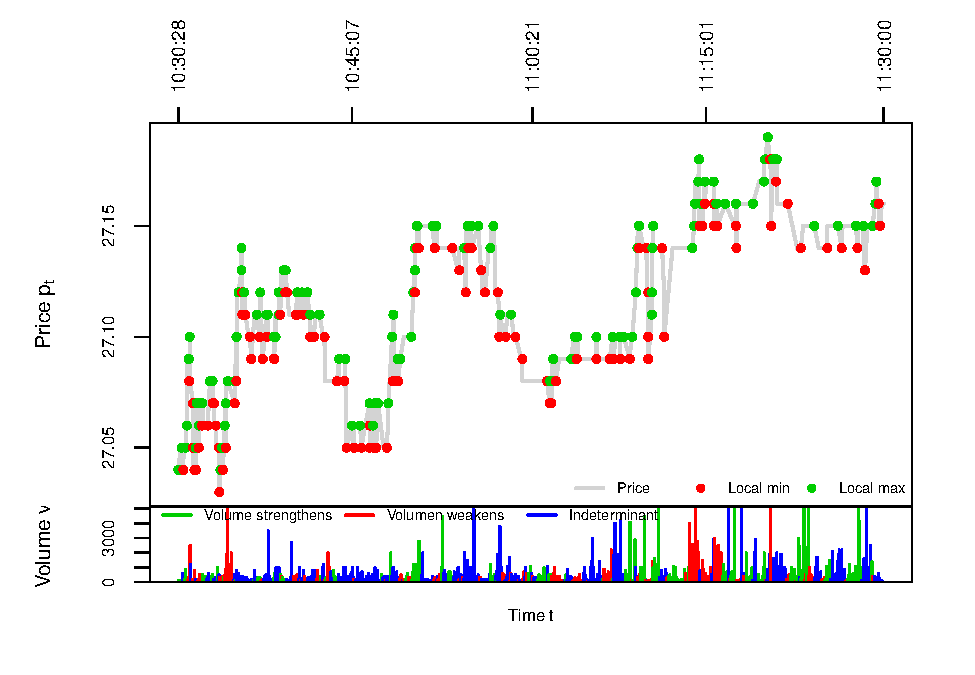
\includegraphics[width=\textwidth,height=0.4 \textheight]{main_files/figure-latex/unnamed-chunk-7-1} \caption{Local extrema detected in TSE:G 2007-05-11 10:30:00/2007-05-11 11:30:00. \label{tseg-ins-extrema}}\label{fig:unnamed-chunk-7}
\end{figure}

\begin{figure}[H]
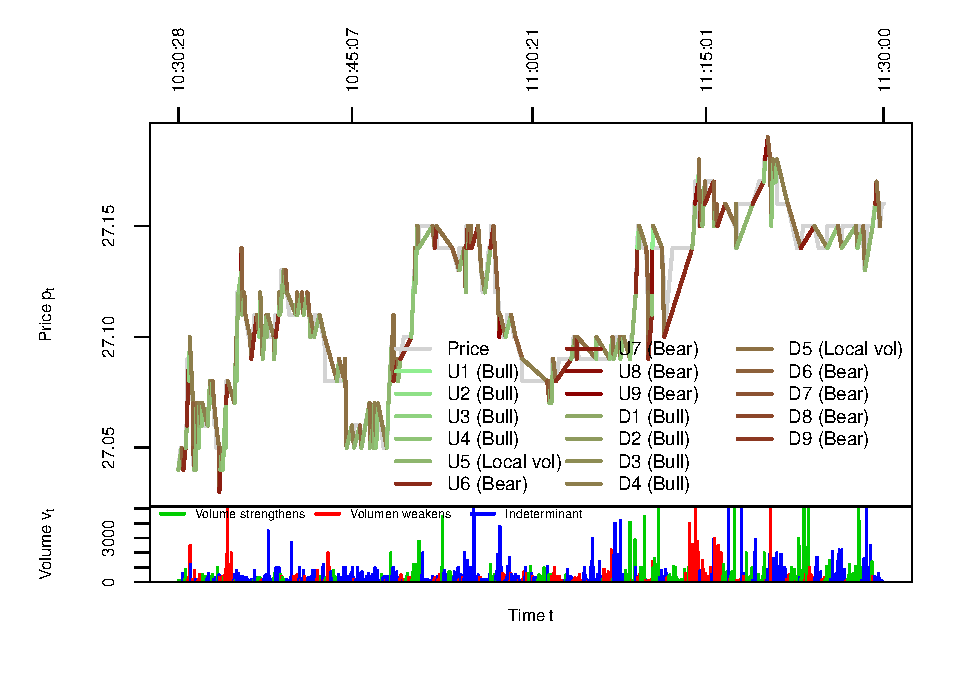
\includegraphics[width=\textwidth,height=0.4 \textheight]{main_files/figure-latex/unnamed-chunk-8-1} \caption{Features extracted from TSE:G 2007-05-11 10:30:00/2007-05-11 11:30:00. \label{tseg-ins-features}}\label{fig:unnamed-chunk-8}
\end{figure}

\subsubsection{Estimation}\label{estimation}

We present a summary of the estimates for the model parameters in
\ref{tab:tseg-ins-params}. The top nodes show some persistence since the
estimated transition probabilities inside \(1 - \\pi_{1}\) and
\(\\pi_{31}\) are close to \(1\). Extreme features are less likely in
all states, which is consistent with our empirical observations.
Features \(D_5\) and \(U_5\) are frequent in both regimens. Features
\(\{D_1, \dots D_4 \}\) are more frequent on the the most frequent
positive and negative legs, are linked to local volatility. ** The
weakness**.

\tiny

\begin{verbatim}
## $xtable.tabular.environment
## NULL
\end{verbatim}

\begin{longtable}[]{@{}rrrrrr@{}}
\caption{\label{tab:tseg-ins-params}}\tabularnewline
\toprule
Parameter & Mean & Std. Deviation & \(q_{10\%}\) & \(q_{50\%}\) &
\(q_{90\%}\)\tabularnewline
\midrule
\endfirsthead
\toprule
Parameter & Mean & Std. Deviation & \(q_{10\%}\) & \(q_{50\%}\) &
\(q_{90\%}\)\tabularnewline
\midrule
\endhead
\(\pi_{1}\) & 0.5067 & 0.282 & 0.0956 & 0.5162 & 0.8931\tabularnewline
\(1 - \pi_{1}\) & 0.4933 & 0.282 & 0.1069 & 0.4838 &
0.9044\tabularnewline
\(a_{12}\) & 0.4559 & 0.1089 & 0.3085 & 0.47 & 0.579\tabularnewline
\(1 - a_{12}\) & 0.5441 & 0.1089 & 0.421 & 0.53 & 0.6915\tabularnewline
\(a_{21}\) & 1 & 0 & 1 & 1 & 1\tabularnewline
\(a_{31}\) & 0.0914 & 0.0623 & 0.0171 & 0.0836 & 0.1717\tabularnewline
\(1 - a_{31}\) & 0.9086 & 0.0623 & 0.8283 & 0.9164 &
0.9829\tabularnewline
\(a_{43}\) & 1 & 0 & 1 & 1 & 1\tabularnewline
\bottomrule
\end{longtable}

\begin{longtable}[]{@{}rrrrrr@{}}
\toprule
Parameter & Mean & Std. Deviation & \(q_{10\%}\) & \(q_{50\%}\) &
\(q_{90\%}\)\tabularnewline
\midrule
\endhead
\(U_1\) & 0.0073 & 0.0057 & 7e-04 & 0.0064 & 0.0152\tabularnewline
\(U_2\) & 0.0196 & 0.0047 & 0.0145 & 0.0188 & 0.0263\tabularnewline
\(U_3\) & 0.0072 & 0.0081 & 6e-04 & 0.0047 & 0.017\tabularnewline
\(U_4\) & 0.3419 & 0.0208 & 0.314 & 0.3436 & 0.3665\tabularnewline
\(U_5\) & 0.2231 & 0.0262 & 0.1873 & 0.2253 & 0.2561\tabularnewline
\(U_6\) & 0.3531 & 0.0174 & 0.3305 & 0.3549 & 0.3719\tabularnewline
\(U_7\) & 0.0264 & 0.0053 & 0.0205 & 0.0263 & 0.0333\tabularnewline
\(U_8\) & 0.0052 & 0.0043 & 6e-04 & 0.0042 & 0.0109\tabularnewline
\(U_9\) & 0.0161 & 0.0046 & 0.0109 & 0.0155 & 0.0226\tabularnewline
\(D_1\) & 0.0017 & 0.0018 & 2e-04 & 0.0011 & 0.004\tabularnewline
\(D_2\) & 0.0226 & 0.0053 & 0.0162 & 0.0223 & 0.0297\tabularnewline
\(D_3\) & 0.0017 & 0.0017 & 1e-04 & 0.0012 & 0.0039\tabularnewline
\(D_4\) & 0.0484 & 0.0333 & 0.0062 & 0.046 & 0.0918\tabularnewline
\(D_5\) & 0.8008 & 0.0403 & 0.7497 & 0.8026 & 0.8528\tabularnewline
\(D_6\) & 0.0236 & 0.0174 & 0.005 & 0.0203 & 0.0469\tabularnewline
\(D_7\) & 0.0796 & 0.008 & 0.0698 & 0.0798 & 0.0891\tabularnewline
\(D_8\) & 0.0011 & 0.001 & 1e-04 & 9e-04 & 0.0023\tabularnewline
\(D_9\) & 0.0205 & 0.0045 & 0.015 & 0.0204 & 0.0262\tabularnewline
\(U_1\) & 0.0105 & 0.0038 & 0.0062 & 0.0106 & 0.0153\tabularnewline
\(U_2\) & 0.0023 & 0.0022 & 3e-04 & 0.0018 & 0.0051\tabularnewline
\(U_3\) & 0.0251 & 0.0052 & 0.0187 & 0.0251 & 0.0314\tabularnewline
\(U_4\) & 0.3554 & 0.0313 & 0.3159 & 0.3549 & 0.3936\tabularnewline
\(U_5\) & 0.1986 & 0.0363 & 0.1525 & 0.1982 & 0.2421\tabularnewline
\(U_6\) & 0.3884 & 0.0198 & 0.3645 & 0.3886 & 0.4154\tabularnewline
\(U_7\) & 0.0023 & 0.0022 & 4e-04 & 0.0017 & 0.0054\tabularnewline
\(U_8\) & 0.0155 & 0.0038 & 0.0111 & 0.015 & 0.0205\tabularnewline
\(U_9\) & 0.0018 & 0.0019 & 2e-04 & 0.0013 & 0.0043\tabularnewline
\(D_1\) & 0.0165 & 0.0066 & 0.007 & 0.017 & 0.0251\tabularnewline
\(D_2\) & 9e-04 & 9e-04 & 1e-04 & 6e-04 & 0.002\tabularnewline
\(D_3\) & 0.0558 & 0.011 & 0.0419 & 0.0574 & 0.0677\tabularnewline
\(D_4\) & 0.0212 & 0.0158 & 0.0044 & 0.0185 & 0.0452\tabularnewline
\(D_5\) & 0.8793 & 0.0237 & 0.8476 & 0.8803 & 0.9057\tabularnewline
\(D_6\) & 0.0132 & 0.0122 & 0.0017 & 0.0088 & 0.0314\tabularnewline
\(D_7\) & 0.0019 & 0.0017 & 3e-04 & 0.0014 & 0.0039\tabularnewline
\(D_8\) & 0.0098 & 0.0052 & 0.0028 & 0.0098 & 0.0168\tabularnewline
\(D_9\) & 0.0014 & 0.0014 & 1e-04 & 9e-04 & 0.0032\tabularnewline
\bottomrule
\end{longtable}

\normalsize

\subsubsection{Convergence}\label{convergence}

Figure \ref{tseg-ins-diags} illustrates the trace plot of some arbitrary
parameters as well as some diagnostic measures. In general terms, mixing
and convergence to the stationary distribution is acceptable. The shrink
factor of \citep{gelman1992inference}, close to \(1\) for all hidden
quantities, indicates an adequate degree of convergence. Sampling is
efficient as signaled by effective sample size ratios near to \(1\) and
Monte Carlo Standar Error to posterior standard deviation ratios well
below 10\%.

\begin{figure}[H]
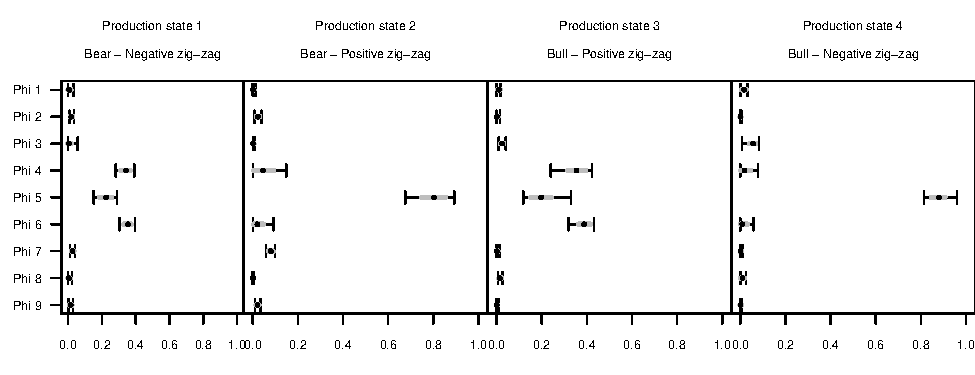
\includegraphics[width=\textwidth]{main_files/figure-latex/unnamed-chunk-11-1} \caption{Traceplot of some arbitrarily selected parameters and histograms of diagnostic measures. Mixing, convergence to the stationary distribution and sampling efficiency are acceptable.\label{tseg-ins-diags}}\label{fig:unnamed-chunk-11}
\end{figure}

Although re-estating the original Hierarchical Hidden Markov Model into
a Hidden Markov Model may increase time and memory complexity, the new
model becomes significantly easier to program and convergence. A full
list of our results, including convergence statistics such as
\(\hat{R}\) and the effective sample size, is included in the appendix.

\subsubsection{State probability}\label{state-probability}

The forward algorithm allows us to calculate the filtered belief state:
the probability that an observation at time \(t\) was emitted by one of
the possible four states (bottom-nodes) given the evidence avaliable up
to \(t\). We assign each observation to the emission state with largest
filtered probability and, by the definition of the hierarchical model,
they become naturally linked to one of the two possible top states
(bears or bulls).

\begin{figure}[H]
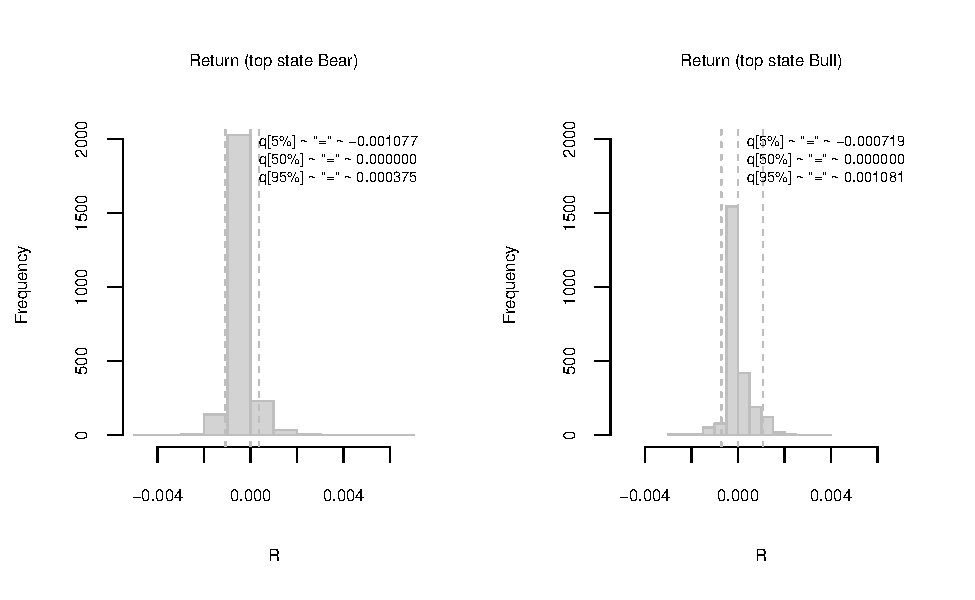
\includegraphics[width=\textwidth]{main_files/figure-latex/unnamed-chunk-13-1} \caption{Distribution of observed features conditional on the estimated hidden regime (top node). \label{tseg-ins-features-hist}}\label{fig:unnamed-chunk-13}
\end{figure}

The following table provides some summary statistics for the returns of
the observations classified in each state. The structure of the top
nodes are symmetrical and they do not have an a priori order. We label
them as runs and reversals according to the expected trade returns
observed in-sample.

\footnotesize

\begin{longtable}[]{@{}llllllllll@{}}
\toprule
Top state & Mean & Std. dev. & Skewness & Kurtosis & \(q_{25}\%\) &
Median & \(q_{75}\%\) & Mean length & Median length\tabularnewline
\midrule
\endhead
Bear & -0.0094 & 0.0648 & 7.9684 & 237.4565 & -0.036 & 0 & 0 & 10.6215 &
6\tabularnewline
Bull & 0.0049 & 0.0515 & 0.9683 & 9.367 & 0 & 0 & 0.0357 & 10.1696 &
6\tabularnewline
Unconditional & -0.0022 & 0.0589 & 5.5346 & 173.8077 & -0.0357 & 0 & 0 &
10.3955 & 6\tabularnewline
\bottomrule
\end{longtable}

\normalsize

Bear and bull top states have negative and positive mean respectively by
construction. As it is also visible in Figure
\ref{fig:tseg-ins-ret-hist}, a positive skewness coefficient for all
states indicates that negative returns tend to overweight positive
returns for this specific stock during the five day long in-sample
dataset. However, bear markets have a marked skew towards negative
returns, becomes more risky in term of extreme events (kurtosis) and
trades in bear markets tend to last one tick more than bulls.

\begin{figure}[H]
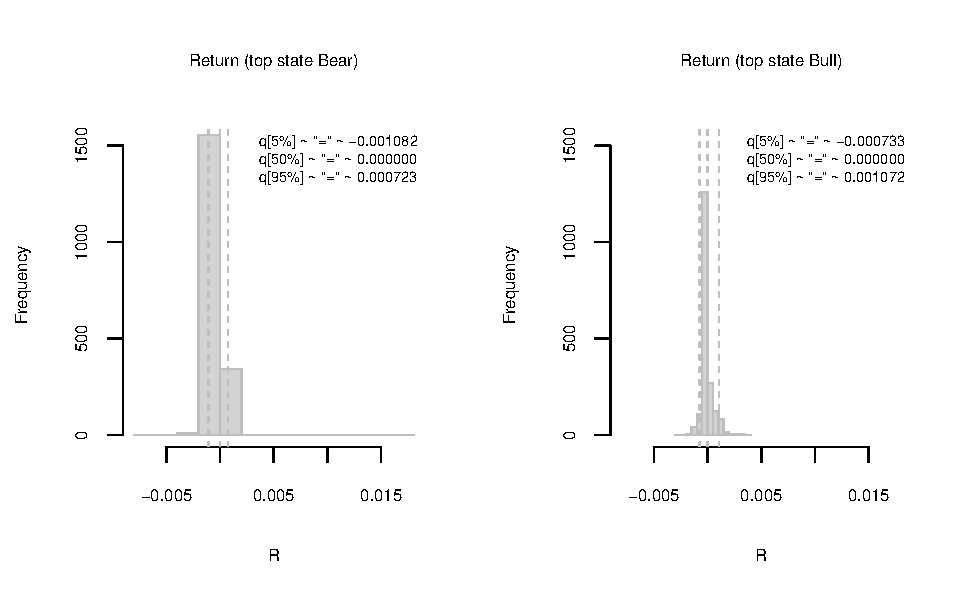
\includegraphics[width=\textwidth]{main_files/figure-latex/unnamed-chunk-15-1} \caption{Conditional distribution of trade returns given the estimated top state in TSE:G 2007-05-04 09:30:00/2007-05-10 16:30:00. \label{fig:tseg-ins-ret-hist}}\label{fig:unnamed-chunk-15}
\end{figure}

We remark that trade returns originated in different stocks or timespans
do not necessarily share these characteristics. Location, dispersion,
symmetry and shape of the returns vary along stocks and day of analysis.

\subsubsection{Fitted output}\label{fitted-output}

As mentioned in Section \ref{sec:model}, the model assumes that outputs
are emitted by one of four possible bottom nodes. By definition,
negative legs belong to either \(z_{1}^2\) or \(z_{4}^2\) while positive
legs belong to \(z_{2}^2\) or \(z_{3}^2\). Once the parameters were
estimated, states \(z_{1}^2\) and \(z_{2}^2\) are labeled as bears while
\(z_{3}^2\) and \(z_{4}^2\) are marked as bulls according to the mean
trade return of the observations included in each of them.

Bullish states allow for negative zig-zags and bearish states allow for
positive zig-zags as long as the trade volume is indeterminant or weak.
The results of the classification are summarized in Table
\ref{tab:tseg-filtered-ins}. As expected, the bullish top-node capture
positive movements due to local volatility as well as downward movements
with weak volume.

Our sampler, tho, maps each of the 18 possible features into one state.
For example, observations from feature 3 (ie U3) are all mapped into
state 4. In a sense, this adds very little information since imputation
is almost deterministic once the parameters are estimated. This is
possibly a weakness in the model.

\tiny

\begin{longtable}[]{@{}rrrrrrrrrrrrrrrrrrrr@{}}
\toprule
Top state & Emission state & \(U_{1}\) & \(U_{2}\) & \(U_{3}\) &
\(U_{4}\) & \(U_{5}\) & \(U_{6}\) & \(U_{7}\) & \(U_{8}\) & \(U_{9}\) &
\(D_{1}\) & \(D_{2}\) & \(D_{3}\) & \(D_{4}\) & \(D_{5}\) & \(D_{6}\) &
\(D_{7}\) & \(D_{8}\) & \(D_{9}\)\tabularnewline
\midrule
\endhead
Bull & \(z^2_{1}\) & 0 & 15 & 0 & 810 & 0 & 828 & 33 & 0 & 17 & 0 & 0 &
0 & 0 & 0 & 0 & 0 & 0 & 0\tabularnewline
Bull & \(z^2_{2}\) & 0 & 0 & 0 & 0 & 0 & 0 & 0 & 0 & 0 & 0 & 72 & 0 & 0
& 2208 & 0 & 181 & 0 & 59\tabularnewline
Bear & \(z^2_{3}\) & 0 & 0 & 0 & 0 & 0 & 0 & 0 & 27 & 0 & 15 & 0 & 34 &
831 & 0 & 846 & 0 & 16 & 0\tabularnewline
Bear & \(z^2_{4}\) & 58 & 0 & 158 & 0 & 2155 & 0 & 0 & 22 & 0 & 0 & 0 &
0 & 0 & 1 & 0 & 0 & 0 & 0\tabularnewline
\bottomrule
\end{longtable}

\normalsize

Now, look how at how the features are classified: Mention plot number on
tayal.

\begin{figure}[H]
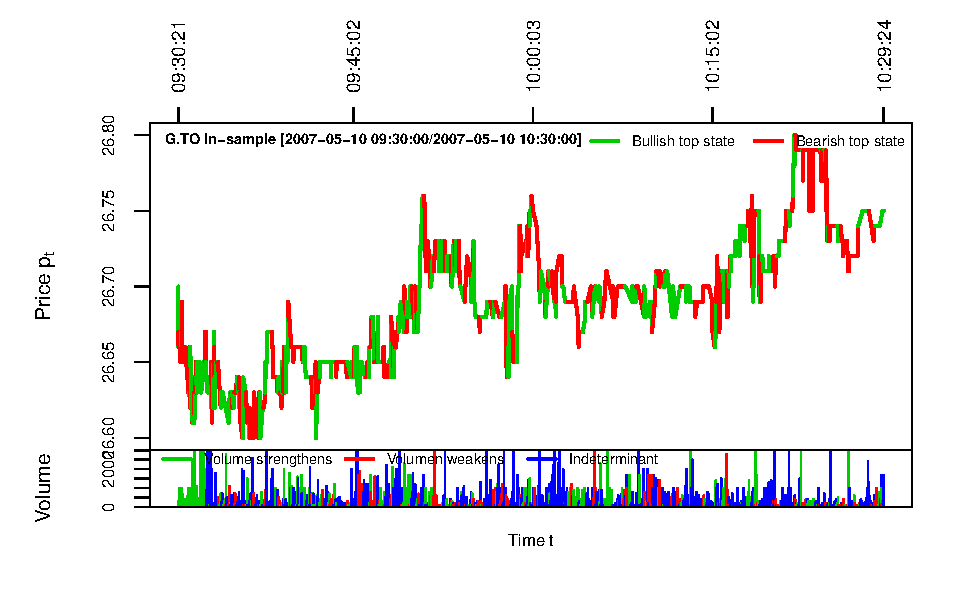
\includegraphics[width=\textwidth]{main_files/figure-latex/unnamed-chunk-17-1} \caption{Tick by tick sequence of trades, classified as belonging to bear or bull states, from TSE:G 2007-05-10 09:30:00/2007-05-10 10:30:00. \label{fig:tseg-ins-seqv}}\label{fig:unnamed-chunk-17}
\end{figure}

\ldots{}

\subsubsection{In-sample summary}\label{in-sample-summary}

\ldots{}

\subsubsection{Forecast}\label{forecast}

\ldots{}

\paragraph{Walking forward forecasts}\label{walking-forward-forecasts}

\ldots{}

\subsubsection{Trading strategy}\label{trading-strategy}

\ldots{}

\subsection{Discussion}\label{further-research}

\subsubsection{The statistical model}\label{the-statistical-model}

\ldots{}

\subsubsection{The financial
application}\label{the-financial-application}

\ldots{}

\begin{center}\rule{0.5\linewidth}{\linethickness}\end{center}

\section{References}\label{references}

\hypertarget{refs}{}

\begin{center}\rule{0.5\linewidth}{\linethickness}\end{center}

\section{Appendix}\label{appendix}

\small

\begin{verbatim}
## Warning in cbind(row.names, mat): number of rows of result is not a
## multiple of vector length (arg 1)
\end{verbatim}

\begin{longtable}[]{@{}rrrrrrrrr@{}}
\toprule
row.names & mean & se\_mean & sd & 10\% & 50\% & 90\% & n\_eff &
Rhat\tabularnewline
\midrule
\endhead
\(\pi_{1}\) & 0.5067 & 0.0178 & 0.282 & 0.0956 & 0.5162 & 0.8931 & 250 &
0.9973\tabularnewline
\(1 - \pi_{1}\) & 0 & 0 & 0 & 0 & 0 & 0 & 250 & NaN\tabularnewline
\(a_{11}\) & 0.4933 & 0.0178 & 0.282 & 0.1069 & 0.4838 & 0.9044 & 250 &
0.9973\tabularnewline
\(a_{12}\) & 0 & 0 & 0 & 0 & 0 & 0 & 250 & NaN\tabularnewline
\(1 - a_{11} - a_{12}\) & 0 & 0 & 0 & 0 & 0 & 0 & 250 &
NaN\tabularnewline
\(a_{22}\) & 0.4559 & 0.0099 & 0.1089 & 0.3085 & 0.47 & 0.579 & 119.7043
& 1.0023\tabularnewline
\(a_{31}\) & 0.5441 & 0.0099 & 0.1089 & 0.421 & 0.53 & 0.6915 & 119.7043
& 1.0023\tabularnewline
\(a_{33}\) & 0 & 0 & 0 & 0 & 0 & 0 & 250 & NaN\tabularnewline
\(1 - a_{31} - a_{33}\) & 1 & 0 & 0 & 1 & 1 & 1 & 250 &
NaN\tabularnewline
\(a_{44}\) & 0 & 0 & 0 & 0 & 0 & 0 & 250 & NaN\tabularnewline
\(\pi_{1}\) & 0 & 0 & 0 & 0 & 0 & 0 & 250 & NaN\tabularnewline
\(1 - \pi_{1}\) & 0 & 0 & 0 & 0 & 0 & 0 & 250 & NaN\tabularnewline
\(a_{11}\) & 0.0914 & 0.0044 & 0.0623 & 0.0171 & 0.0836 & 0.1717 &
198.8658 & 0.9998\tabularnewline
\(a_{12}\) & 0 & 0 & 0 & 0 & 0 & 0 & 250 & NaN\tabularnewline
\(1 - a_{11} - a_{12}\) & 0 & 0 & 0 & 0 & 0 & 0 & 250 &
NaN\tabularnewline
\(a_{22}\) & 0.9086 & 0.0044 & 0.0623 & 0.8283 & 0.9164 & 0.9829 &
198.8658 & 0.9998\tabularnewline
\(a_{31}\) & 0 & 0 & 0 & 0 & 0 & 0 & 250 & NaN\tabularnewline
\(a_{33}\) & 0 & 0 & 0 & 0 & 0 & 0 & 250 & NaN\tabularnewline
\(1 - a_{31} - a_{33}\) & 1 & 0 & 0 & 1 & 1 & 1 & 250 &
NaN\tabularnewline
\(a_{44}\) & 0 & 0 & 0 & 0 & 0 & 0 & 250 & NaN\tabularnewline
\(\pi_{1}\) & 0.0073 & 6e-04 & 0.0057 & 7e-04 & 0.0064 & 0.0152 &
99.4159 & 1.0095\tabularnewline
\(1 - \pi_{1}\) & 0.0196 & 3e-04 & 0.0047 & 0.0145 & 0.0188 & 0.0263 &
250 & 0.997\tabularnewline
\(a_{11}\) & 0.0072 & 8e-04 & 0.0081 & 6e-04 & 0.0047 & 0.017 & 102.0471
& 1.0182\tabularnewline
\(a_{12}\) & 0.3419 & 0.0017 & 0.0208 & 0.314 & 0.3436 & 0.3665 &
150.0721 & 1.0051\tabularnewline
\(1 - a_{11} - a_{12}\) & 0.2231 & 0.002 & 0.0262 & 0.1873 & 0.2253 &
0.2561 & 171.5795 & 1.0062\tabularnewline
\(a_{22}\) & 0.3531 & 0.0011 & 0.0174 & 0.3305 & 0.3549 & 0.3719 & 250 &
0.9962\tabularnewline
\(a_{31}\) & 0.0264 & 3e-04 & 0.0053 & 0.0205 & 0.0263 & 0.0333 & 250 &
0.9963\tabularnewline
\(a_{33}\) & 0.0052 & 4e-04 & 0.0043 & 6e-04 & 0.0042 & 0.0109 &
144.0005 & 0.9979\tabularnewline
\(1 - a_{31} - a_{33}\) & 0.0161 & 3e-04 & 0.0046 & 0.0109 & 0.0155 &
0.0226 & 250 & 0.9997\tabularnewline
\(a_{44}\) & 0.0017 & 2e-04 & 0.0018 & 2e-04 & 0.0011 & 0.004 & 66.4428
& 1.0057\tabularnewline
\(\pi_{1}\) & 0.0226 & 3e-04 & 0.0053 & 0.0162 & 0.0223 & 0.0297 & 250 &
1.0017\tabularnewline
\(1 - \pi_{1}\) & 0.0017 & 1e-04 & 0.0017 & 1e-04 & 0.0012 & 0.0039 &
250 & 0.9993\tabularnewline
\(a_{11}\) & 0.0484 & 0.0033 & 0.0333 & 0.0062 & 0.046 & 0.0918 &
102.2995 & 0.9976\tabularnewline
\(a_{12}\) & 0.8008 & 0.0042 & 0.0403 & 0.7497 & 0.8026 & 0.8528 &
90.8209 & 0.9961\tabularnewline
\(1 - a_{11} - a_{12}\) & 0.0236 & 0.0012 & 0.0174 & 0.005 & 0.0203 &
0.0469 & 194.2454 & 0.997\tabularnewline
\(a_{22}\) & 0.0796 & 5e-04 & 0.008 & 0.0698 & 0.0798 & 0.0891 & 250 &
0.9962\tabularnewline
\(a_{31}\) & 0.0011 & 1e-04 & 0.001 & 1e-04 & 9e-04 & 0.0023 & 250 &
0.9961\tabularnewline
\(a_{33}\) & 0.0205 & 3e-04 & 0.0045 & 0.015 & 0.0204 & 0.0262 & 250 &
0.9965\tabularnewline
\(1 - a_{31} - a_{33}\) & 0.0105 & 5e-04 & 0.0038 & 0.0062 & 0.0106 &
0.0153 & 52.9642 & 0.9989\tabularnewline
\(a_{44}\) & 0.0023 & 1e-04 & 0.0022 & 3e-04 & 0.0018 & 0.0051 & 250 &
0.996\tabularnewline
\(\pi_{1}\) & 0.0251 & 3e-04 & 0.0052 & 0.0187 & 0.0251 & 0.0314 & 250 &
0.9964\tabularnewline
\(1 - \pi_{1}\) & 0.3554 & 0.003 & 0.0313 & 0.3159 & 0.3549 & 0.3936 &
111.4928 & 0.9961\tabularnewline
\(a_{11}\) & 0.1986 & 0.0036 & 0.0363 & 0.1525 & 0.1982 & 0.2421 &
99.991 & 0.9961\tabularnewline
\(a_{12}\) & 0.3884 & 0.0013 & 0.0198 & 0.3645 & 0.3886 & 0.4154 &
227.1397 & 0.9964\tabularnewline
\(1 - a_{11} - a_{12}\) & 0.0023 & 1e-04 & 0.0022 & 4e-04 & 0.0017 &
0.0054 & 250 & 0.996\tabularnewline
\(a_{22}\) & 0.0155 & 2e-04 & 0.0038 & 0.0111 & 0.015 & 0.0205 & 250 &
0.996\tabularnewline
\(a_{31}\) & 0.0018 & 1e-04 & 0.0019 & 2e-04 & 0.0013 & 0.0043 & 250 &
0.9962\tabularnewline
\(a_{33}\) & 0.0165 & 8e-04 & 0.0066 & 0.007 & 0.017 & 0.0251 & 75.1274
& 1.0015\tabularnewline
\(1 - a_{31} - a_{33}\) & 9e-04 & 1e-04 & 9e-04 & 1e-04 & 6e-04 & 0.002
& 250 & 0.9983\tabularnewline
\(a_{44}\) & 0.0558 & 0.001 & 0.011 & 0.0419 & 0.0574 & 0.0677 &
124.3395 & 1.0162\tabularnewline
\(\pi_{1}\) & 0.0212 & 0.0012 & 0.0158 & 0.0044 & 0.0185 & 0.0452 &
178.8572 & 1.0063\tabularnewline
\(1 - \pi_{1}\) & 0.8793 & 0.0023 & 0.0237 & 0.8476 & 0.8803 & 0.9057 &
110.8629 & 1.0212\tabularnewline
\(a_{11}\) & 0.0132 & 0.001 & 0.0122 & 0.0017 & 0.0088 & 0.0314 &
151.8973 & 1.0038\tabularnewline
\(a_{12}\) & 0.0019 & 1e-04 & 0.0017 & 3e-04 & 0.0014 & 0.0039 & 250 &
0.9966\tabularnewline
\(1 - a_{11} - a_{12}\) & 0.0098 & 5e-04 & 0.0052 & 0.0028 & 0.0098 &
0.0168 & 110.7242 & 0.9962\tabularnewline
\(a_{22}\) & 0.0014 & 1e-04 & 0.0014 & 1e-04 & 9e-04 & 0.0032 & 250 &
0.9991\tabularnewline
\normalsize & & & & & & & &\tabularnewline
\bottomrule
\end{longtable}

\renewcommand\refname{Original Computing Environment}
\bibliography{../common/references}


\end{document}
